\chapter{Opis algorytmu symulowanego wyżarzania} \label{chapter:sa-desc}
\label{annealing}
Symulowane wyżarzanie \cite{metaheuristic-handbook} (z ang.\emph{simulated annealing}) (w skrócie: SA) jest metaheurystyką stosowaną, przy rozwiązywaniu szerokiego wachlarza problemów \emph{NP trudnych}. W tym rozdziale opisane zostaną kluczowe elementy składowe SA takie jak: funkcja celu, ograniczenia, schemat chłodzenia itd.

\section{Schemat działania symulowanego wyżarzania}

\begin{algorithm}
\caption{Symulowane wyżarzanie}
\label{alg-annealing}
\begin{algorithmic}[1]
\Procedure{$SA$}{$sol, initialTemp$}
\State $temp\gets initialTemp$\Comment{Temperatura początkowa}
\State $bestSol\gets sol$\Comment{Najlepsze rozwiązanie}
\State $beforeChange\gets sol$\Comment{Rozwiązanie przed zmianą}
\While{$stopCriteria()\not=true$}
\State $beforeChange \gets sol$\Comment{Zachowaj kopię rozwiązania przed zmianą}
\State $Change(sol)$\Comment{Zmień rozwiązanie i oceń je}
\State $Eval(sol)$
\State $diff \gets Diff(sol,solChange)$
\If{$sol.Value > beforeChange.Value$ \textbf{or} $rand() < exp(\frac{diff}{temp})$}
\If{$sol.Value > bestSol.Value$}\label{annealing-comp}
\State$bestSol \gets sol$
\EndIf
\Else
\State $sol \gets beforeChange$\label{annealing-copy}
\EndIf
\State$Cool(temp)$\Comment{Zmień temperaturę}
\EndWhile
\State $\textbf{return}\ bestSol$
\EndProcedure
\end{algorithmic}
\end{algorithm}
\newpage
Jak widać na schemacie, symulowane wyżarzanie nieco przypomina algorytm
genetyczny. Jest to jednak podobieństwo powierzchowne. Obie heurystyki działają
w pętli $while$. Warunkiem wyjścia z pętli może być maksymalna ilość kroków,
brak znalezienia lepszego rozwiązania przez pewien czas, czy osiągnięcie
minimalnej temperatury. Podczas trwania głównej pętli $while$ algorytm
zapamiętuje trzy rozwiązania:
\begin{itemize}
	\item $bestSol$ - najlepsze napotkane rozwiązanie.
	\item $beforeChange$ - rozwiązanie przed zmianą, będące punktem
		powrotnym w przypadku niefortunnej zmiany rozwiązania.
	\item $sol$ - aktywnie zmieniane rozwiązanie.
\end{itemize}
Po zmianie rozwiązania ($Change(sol)$) następuje ocena ($Eval(sol)$). Jeśli
wartość rozwiązania po zmianie jest większa niż przed lub jeśli temperatura jest
dostatecznie wysoka aby na taką zmianę pozwolić, wtedy algorytm zapamiętuje
rozwiązanie $sol$ jako punk wyjścia do następnego ruchu (linia 10). Jeśli zmienione
rozwiązanie $sol$ zostanie odrzucone, wtedy jako punk wyjścia do dalszych zmian
posłuży stara wersja rozwiązania (linia 15).

Jeśli nowe rozwiązanie polepszyło się na skutek ruchu, wtedy możemy sprawdzić
czy jest lepsze niż najlepsze napotkane do tej pory (linia 11). Jeśli tak, to
jest ono zapamiętywane jako takie.

\section{Tworzenie rozwiązanie początkowego}
To jakie rozwiązanie początkowe otrzyma algorytm zależy ściśle od specyfiki
problemu. To od charakterystyki rozwiązania początkowego uzależniony jest etap
doboru parametrów. Jeśli rozwiązanie początkowe jest dobrej jakości, to
temperatura początkowa musi być wysoka aby pozwolić algorytmowi na wyjście poza
krąg sąsiednich rozwiązań, które najprawdopodobniej są gorsze od początkowego.

Jeśli rozwiązanie początkowe jest bardzo oddalone od rejonu przestrzeni
rozwiązań w którym podejrzewamy, że znajduje się optymalne rozwiązanie, wtedy
niska temperatura początkowa pozwali szybko zbliżyć się do tego miejsca. Szybkie
zbliżenie do bardzo konkretnego rejonu przestrzeni rozwiązań, może mieć zgubny
wpływ na szansę znalezienia lepszego rozwiązania, które znajduje się w innej
jego części.

\section{Sposoby zmiany rozwiązania}
Funkcja $Change(sol)$ reprezentuje zmianę rozwiązania. To jak przebiega zmiana
rozwiązania zależy od specyfiki problemu. Ważne aby zmiana rozwiązania była uzależniona
od stanu poprzedniego.
Często spotykaną formą zmiany rozwiązania w problemie harmonogramowania, jest
zmiana przypisania wydarzenia do terminu. Nowy termin może zostać wybrany losowo
lub za pomocą pomocniczych funkcji przeszukiwania lokalnego (z ang.
\emph{local search}).
\newpage
\section{Specyfika funkcji oceny}
Funkcja oceny $Eval(sol)$ przypisuje wartość ocenianemu rozwiązaniu. Funkcja ta
może obliczyć wartość rozwiązania na dwa sposoby:
\begin{itemize}
	\item Wartość jako suma kary za niedopuszczalność i wartości za
		spełnienie preferencji.
	\item Wartość jako kara za niedopuszczalność lub wartości za
		spełnienie preferencji.
\end{itemize}
Karą w problemach harmonogramowania może być liczba wydarzeń, które nie mają
przypisanego bezkonfliktowego terminu a np. w problemie plecakowym różnica między
pojemnością plecaka a rzeczywistą wagą zabranych przedmiotów.

Wartością naliczaną za spełnienie preferencji może być różnica między
najwcześniejszym terminem w ciągu dnia a tym najpóźniejszym. Im mniejsza różnica
tym lepiej. Dzięki temu premiujemy rozwiązania bardziej "ściśnięte".

\section{Wpływ temperatury na akceptację rozwiązania}
Algorytm SA tym różni się od algorytmu wspinaczkowego (z ang. \emph{hill
climbing algorithm}), że pozwala na ruch pogarszający. To czy taki ruch
pogarszający będzie miał miejsce czy też nie zależy od aktualnej temperatury. Im
większa temperatura, tym większe prawdopodobieństwo akceptacji rozwiązania
niedopuszczalnego. Ten prosty mechanizm pozwala algorytmowi pokonywać lokalne
minima i maksima z którymi algorytm wspinaczkowy nie jest sobie w stanie
poradzić.

\section{Schematy chłodzenia}
Podobnie jak przy poprzednich elementach algorytmu, schemat chłodzenia ściśle
zależy od rozwiązywanego problemu. Im mniejsza temperatura, tym mniejsze
prawdopodobieństwo akceptacji ruchu pogarszającego. Delikatne obniżanie
temperatury pozwoli na zbadanie większej części przestrzeni rozwiązań. Niewielka
temperatura nie pozwoli na powędrowanie w rejony przestrzeni rozwiązań, znacząco
oddalone od punktu w którym znajduje się rozwiązanie początkowe.

\begin{figure}[!h]
	\centering
\begin{tabular}{ c c }
	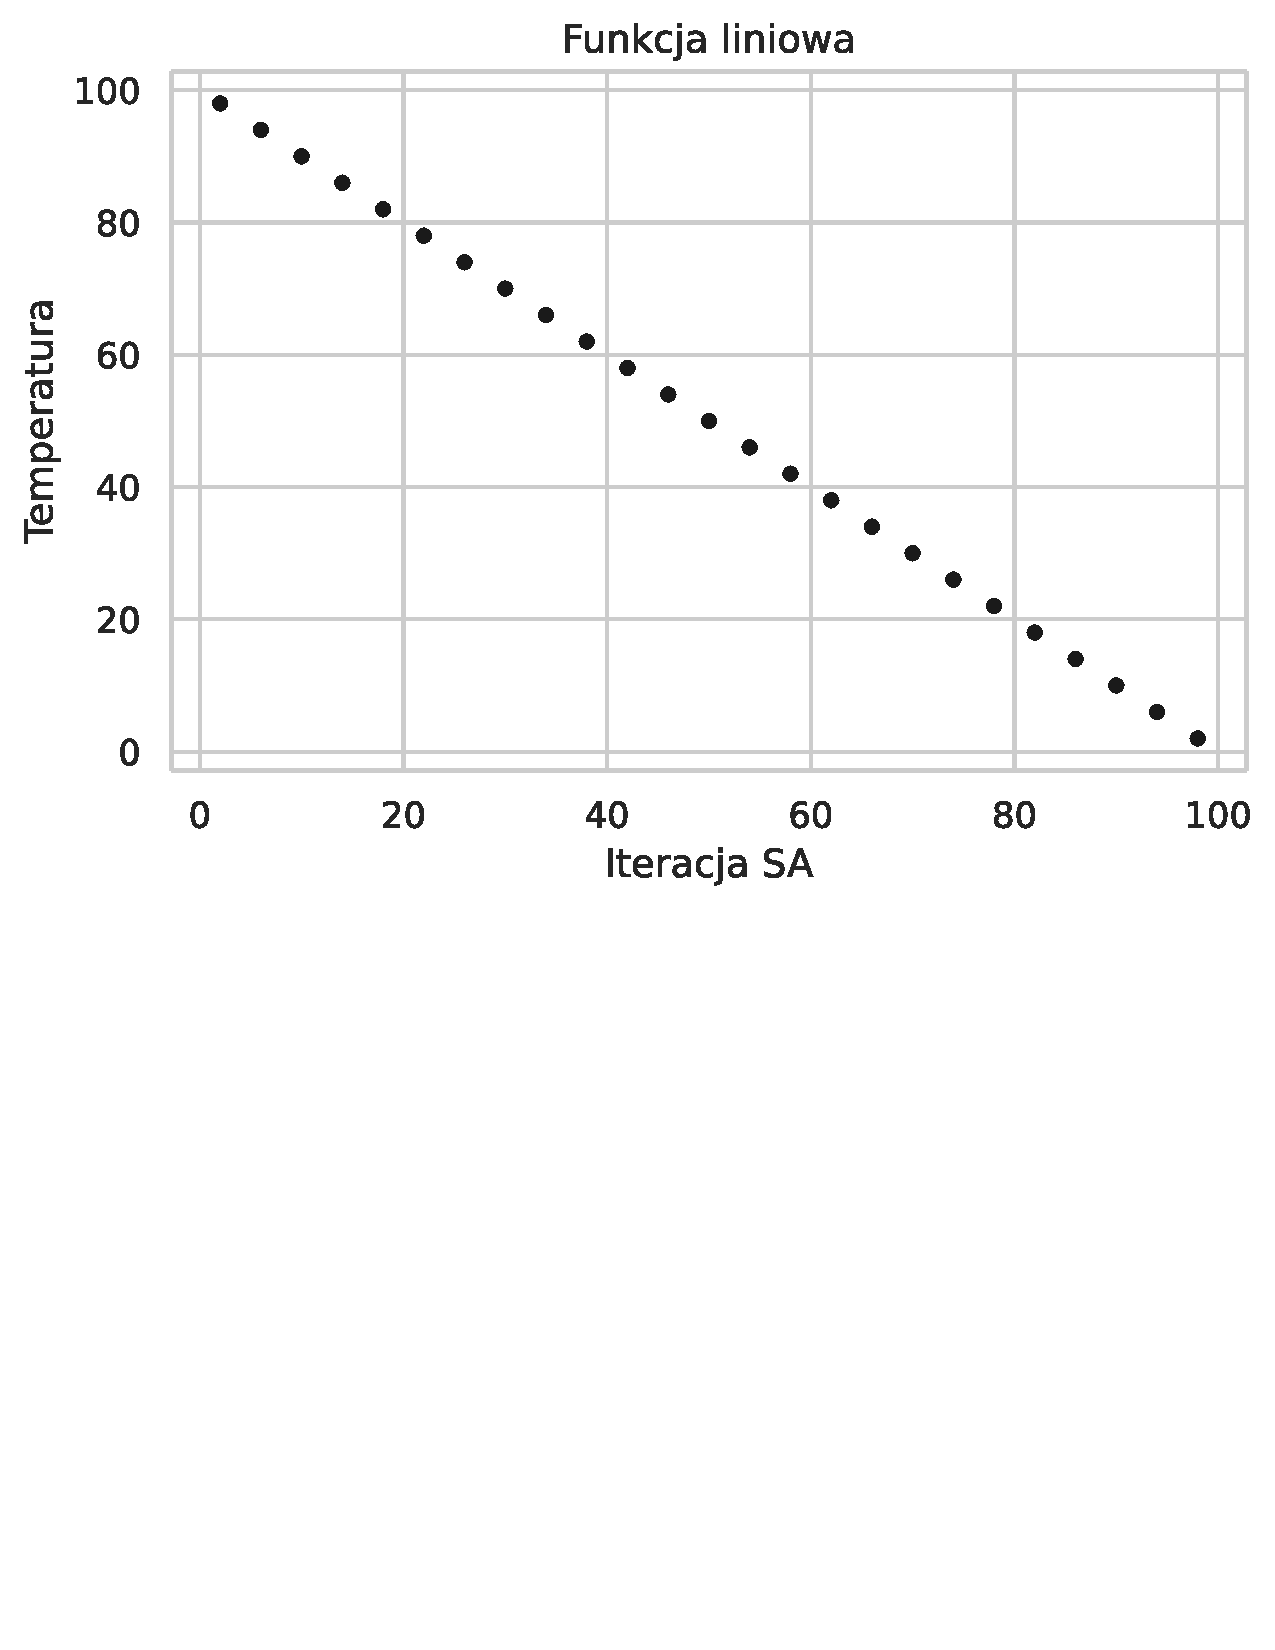
\includegraphics[width=0.5\textwidth]{gfx/temp_linear.pdf} & 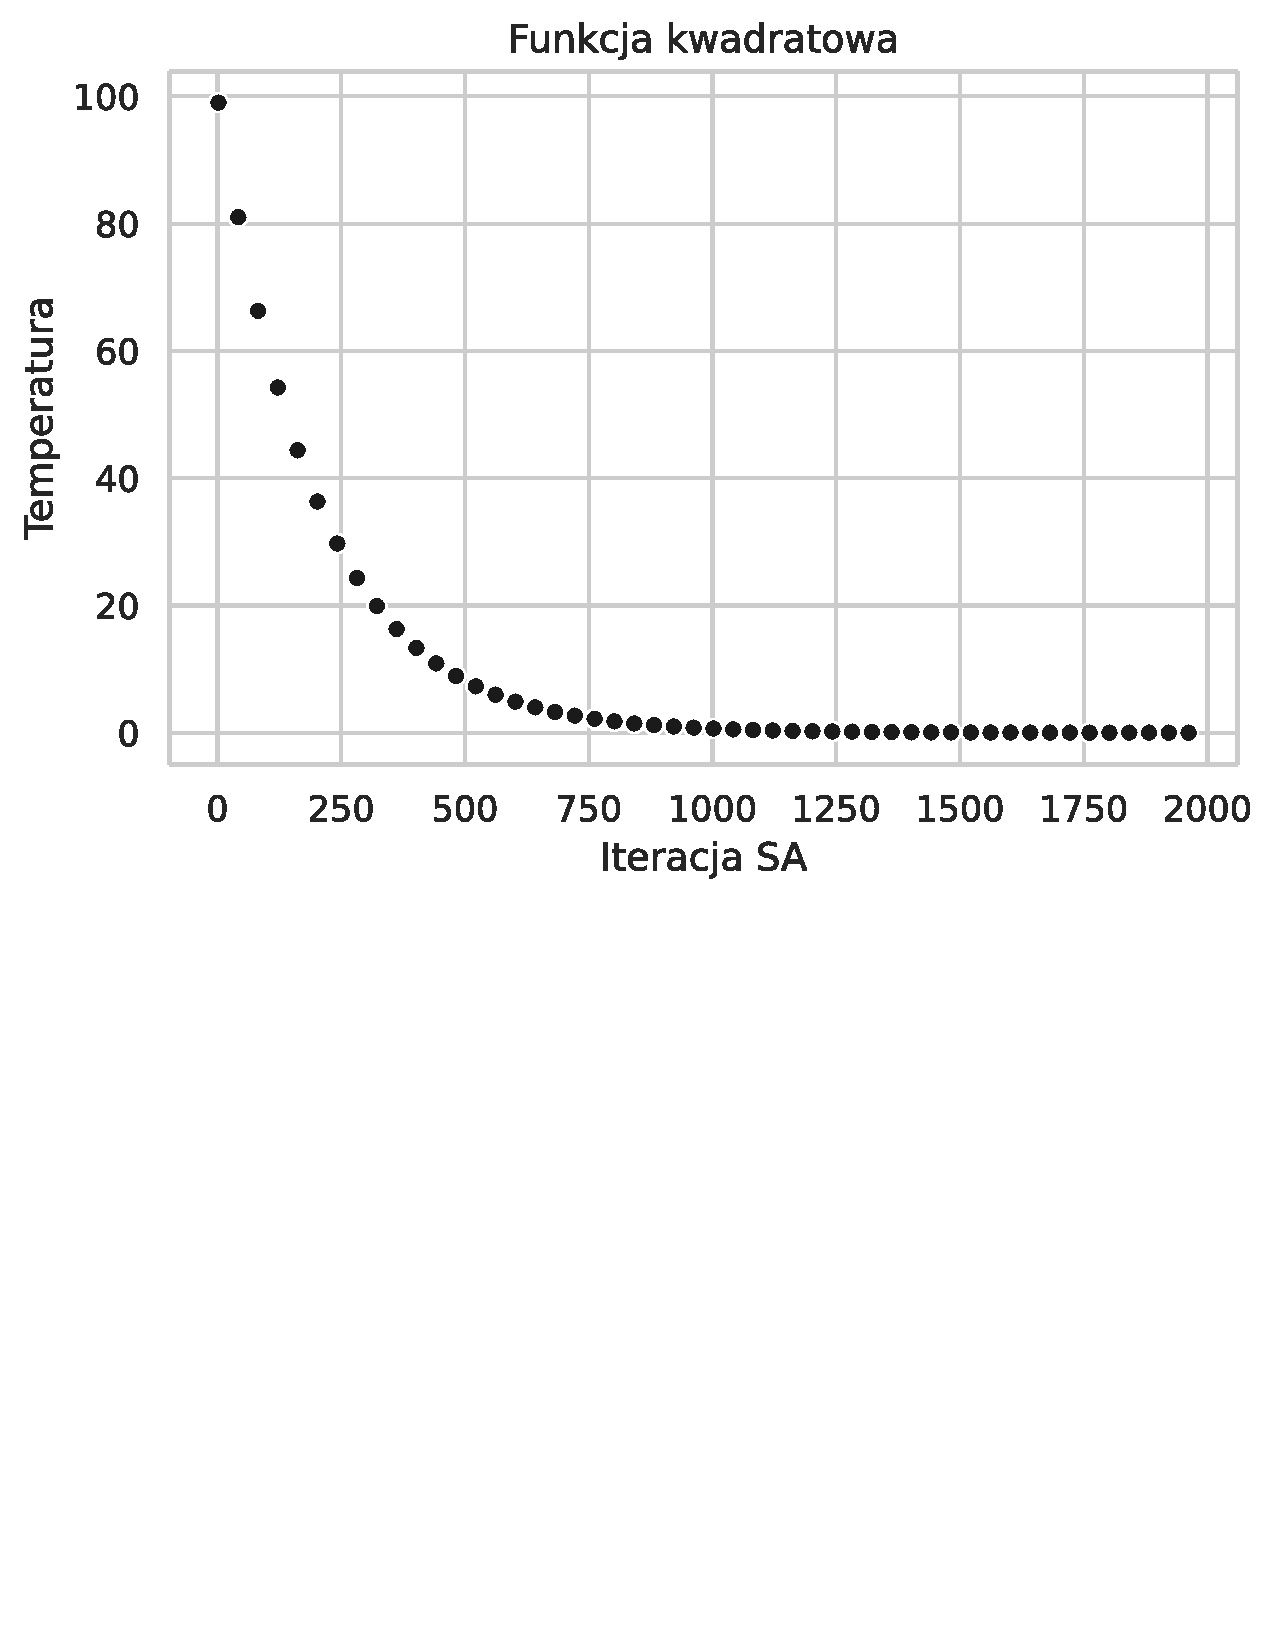
\includegraphics[width=0.5\textwidth]{gfx/temp_quadriatic.pdf} \\
	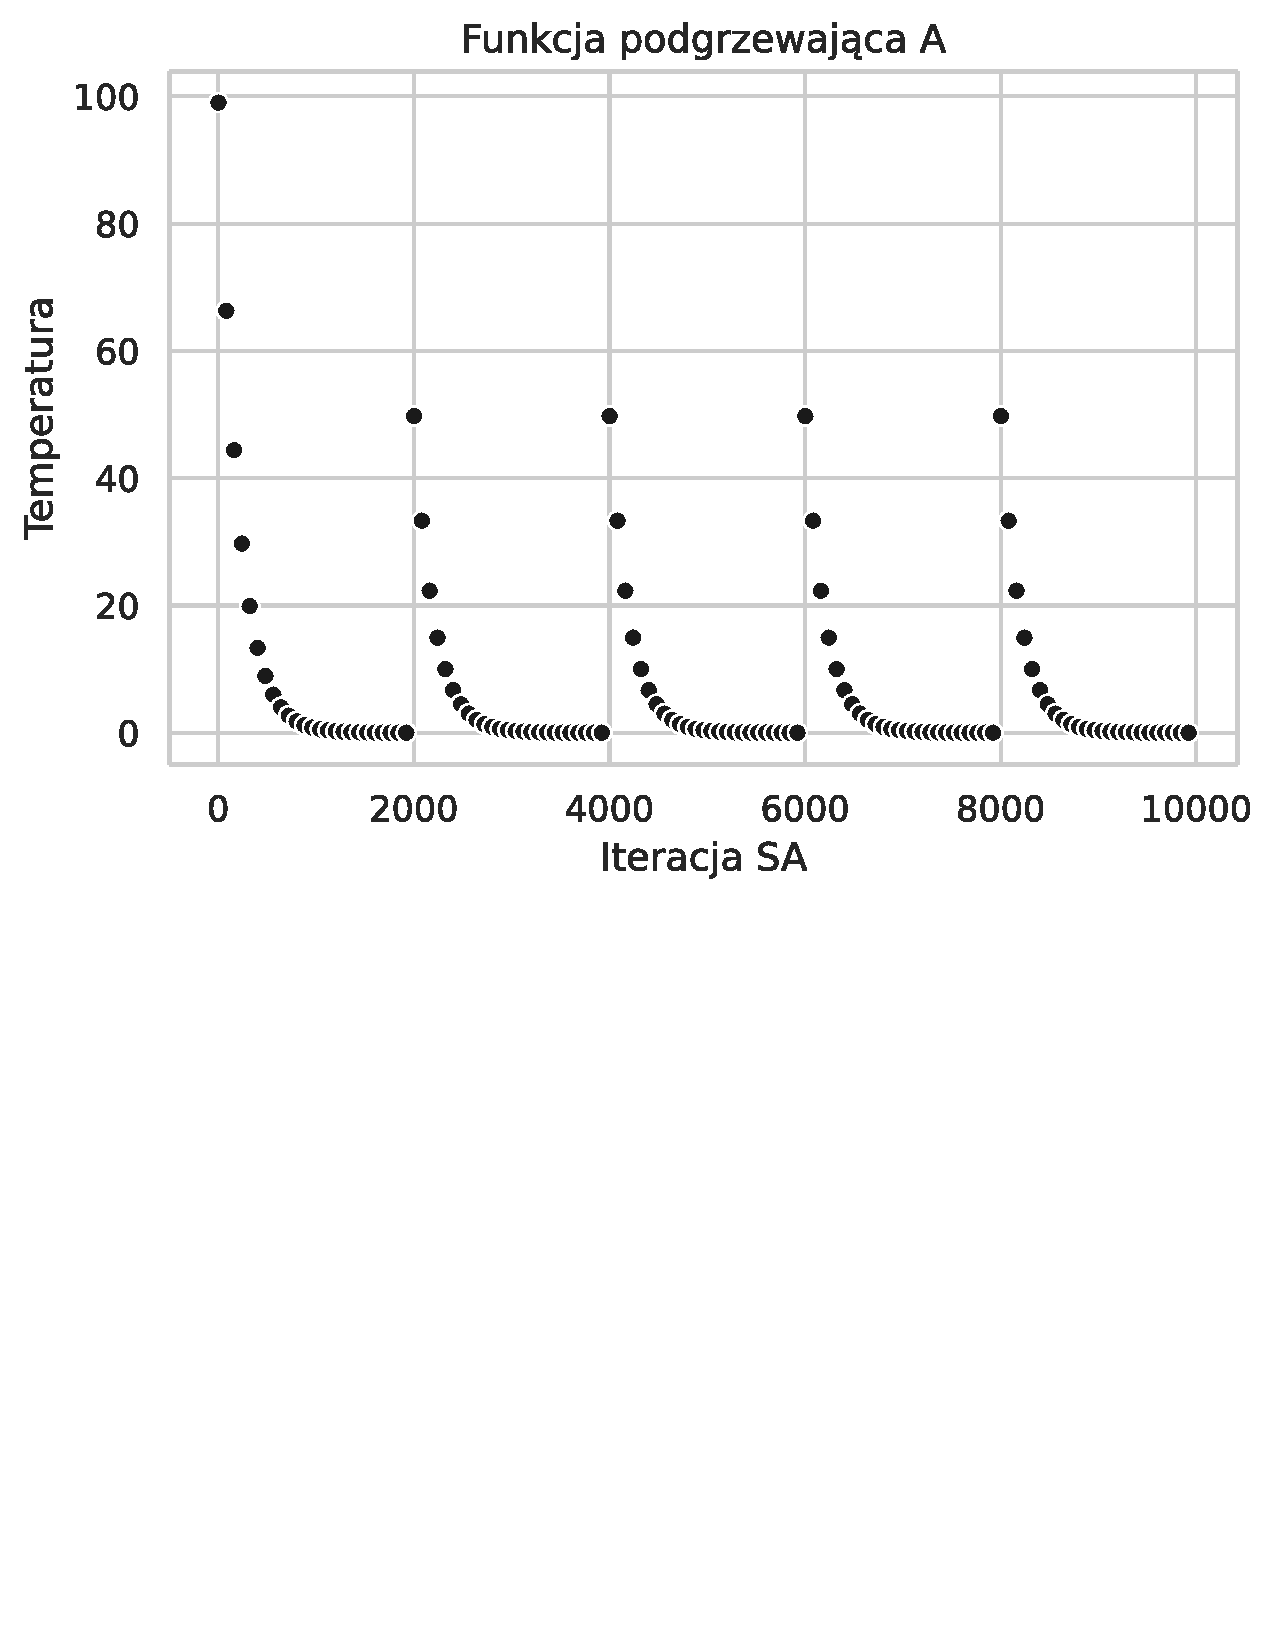
\includegraphics[width=0.5\textwidth]{gfx/temp_heater_a.pdf} & 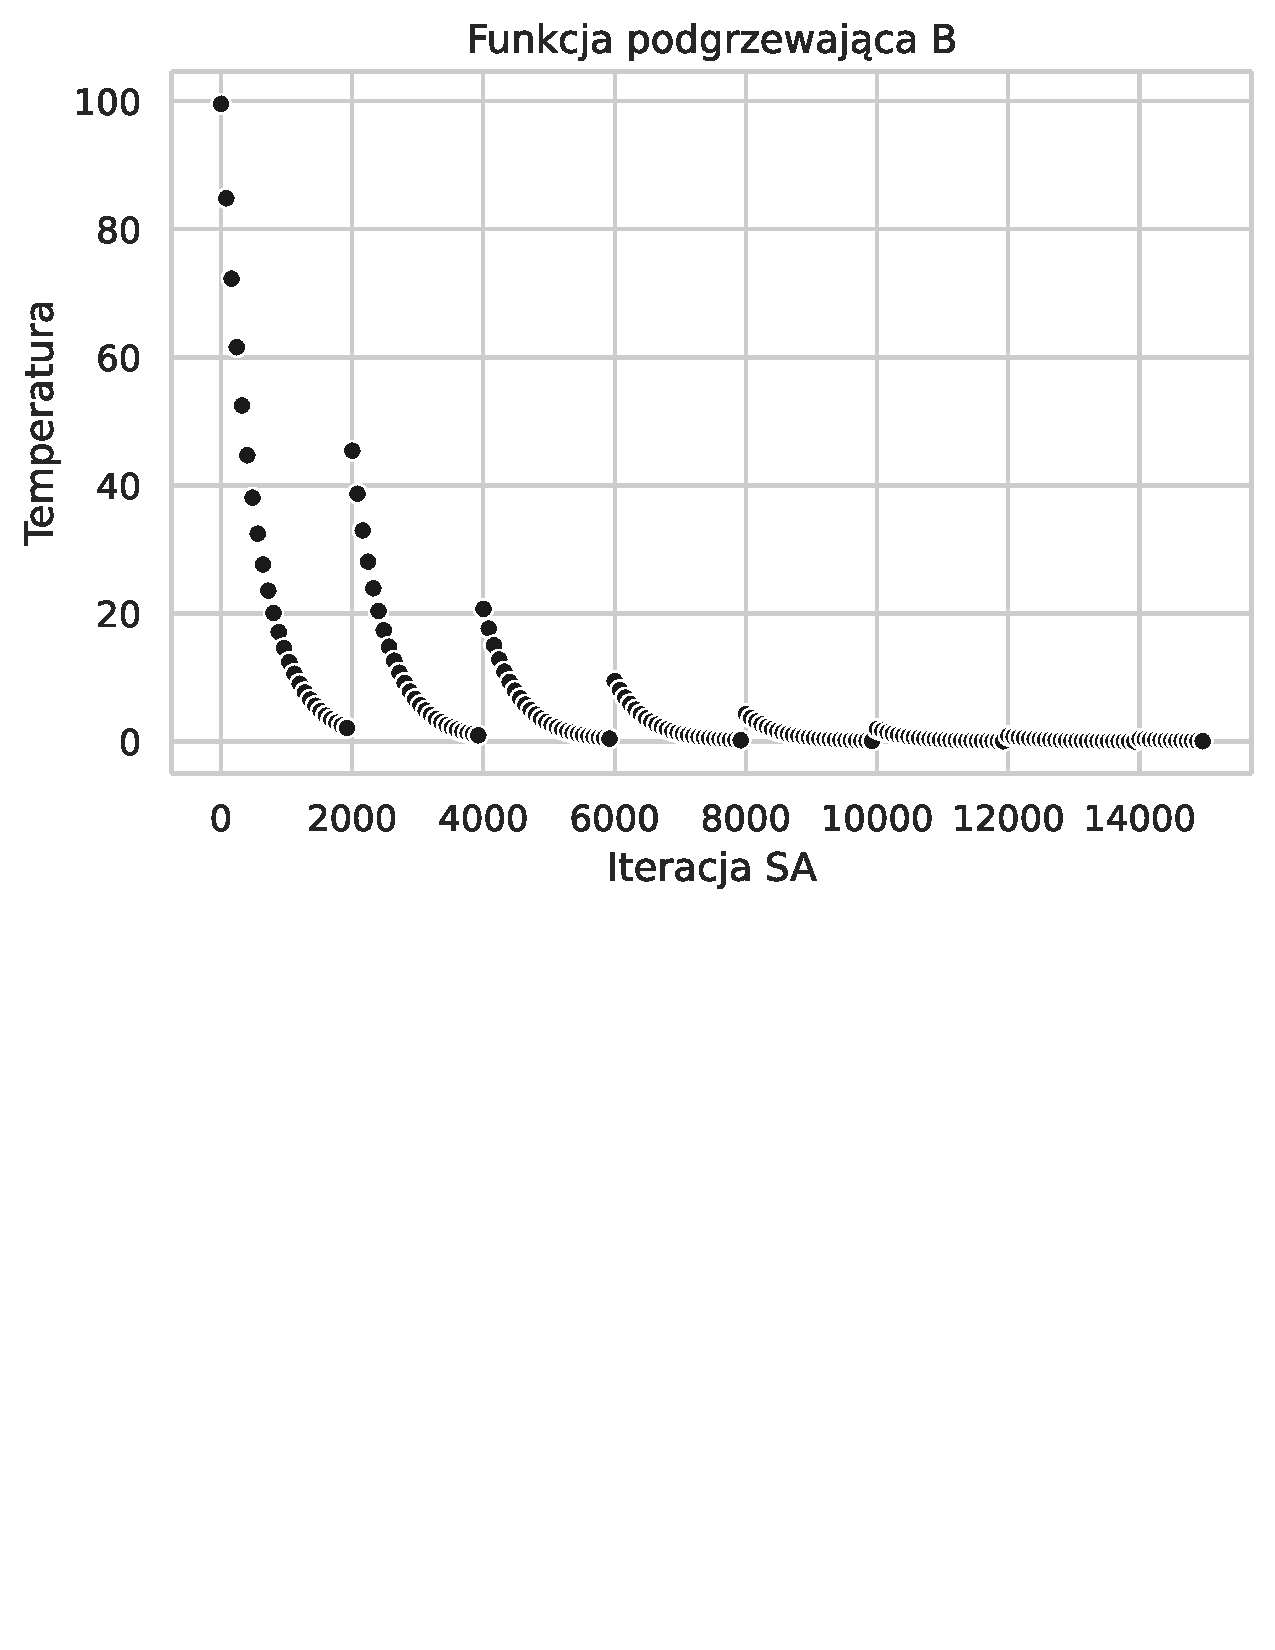
\includegraphics[width=0.5\textwidth]{gfx/temp_heater_b.pdf}
\end{tabular}
	\caption{Przykładowe funkcje obniżające temperaturę}
	\label{example-cooling-functions}
\end{figure}
\newpage
\section{Kryteria stopu}
\label{sec:stop-criteria}
Algorytm działa w pętli $while$ która ulega przerwaniu jeśli spełniony zostanie
warunek stopu. Jeśli nie wykorzystujemy algorytmu w wersji online czyli takiej,
która ciągle, na bieżąco stara się znaleźć najlepsze rozwiązanie przy
zmieniającym się krajobrazie funkcji celu, wtedy możemy zastosować jeden z
poniższych warunków:

\subsubsection{Maksymalna ilość kroków} 
Podstawowy warunek stopu. Algorytm przerwie działanie jeśli dotrze do danej
iteracji pętli $while$. Istnieje ryzyko, że algorytm będzie działał nawet po
znalezieniu dobrego rozwiązania, lub braku znaczącej poprawy w jakości
uzyskiwanych rozwiązań. Jeśli nasz problem ma styczność z dużym spektrum
skomplikowania instancji problemu, wtedy wykorzystanie tylko tego warunku nie jest
dobrym pomysłem.

\subsubsection{Maksymalny czas} 
Algorytm będzie działa tylko przez określony czas
np. 2 godziny. Uwagi i problemu związane z tym kryterium są analogiczne do tych
z warunku poprzedniego.

\subsubsection{Minimalna wartość} 
Algorytm przerwie działanie, po znalezieniu rozwiązania o pewnej minimalnej
wartości. Ten warunek musi zostać połączony z innym kryterium stopu, ponieważ
istnieje ryzyko nieznalezienia rozwiązania o wymaganej wartości.

\subsubsection{Maksymalny czas bez poprawy} 
Algorytm przerywa pętlę, jeśli przez określony czas np. ilość iteracji algorytm
nie znalazł rozwiązania, które byłoby lepsze niż najlepsze do tej pory
znalezione ($bestSol$). Można lekko zmodyfikować ten warunek i określić minimalną
różnicę między rozwiązaniami, która będzie traktowana jako polepszenie. 
